% Created 2021-09-27 Mon 12:02
% Intended LaTeX compiler: xelatex
\documentclass[letterpaper]{article}
\usepackage{graphicx}
\usepackage{grffile}
\usepackage{longtable}
\usepackage{wrapfig}
\usepackage{rotating}
\usepackage[normalem]{ulem}
\usepackage{amsmath}
\usepackage{textcomp}
\usepackage{amssymb}
\usepackage{capt-of}
\usepackage{hyperref}
\setlength{\parindent}{0pt}
\usepackage[margin=1in]{geometry}
\usepackage{fontspec}
\usepackage{svg}
\usepackage{cancel}
\usepackage{indentfirst}
\setmainfont[ItalicFont = LiberationSans-Italic, BoldFont = LiberationSans-Bold, BoldItalicFont = LiberationSans-BoldItalic]{LiberationSans}
\newfontfamily\NHLight[ItalicFont = LiberationSansNarrow-Italic, BoldFont       = LiberationSansNarrow-Bold, BoldItalicFont = LiberationSansNarrow-BoldItalic]{LiberationSansNarrow}
\newcommand\textrmlf[1]{{\NHLight#1}}
\newcommand\textitlf[1]{{\NHLight\itshape#1}}
\let\textbflf\textrm
\newcommand\textulf[1]{{\NHLight\bfseries#1}}
\newcommand\textuitlf[1]{{\NHLight\bfseries\itshape#1}}
\usepackage{fancyhdr}
\pagestyle{fancy}
\usepackage{titlesec}
\usepackage{titling}
\makeatletter
\lhead{\textbf{\@title}}
\makeatother
\rhead{\textrmlf{Compiled} \today}
\lfoot{\theauthor\ \textbullet \ \textbf{2021-2022}}
\cfoot{}
\rfoot{\textrmlf{Page} \thepage}
\renewcommand{\tableofcontents}{}
\titleformat{\section} {\Large} {\textrmlf{\thesection} {|}} {0.3em} {\textbf}
\titleformat{\subsection} {\large} {\textrmlf{\thesubsection} {|}} {0.2em} {\textbf}
\titleformat{\subsubsection} {\large} {\textrmlf{\thesubsubsection} {|}} {0.1em} {\textbf}
\setlength{\parskip}{0.45em}
\renewcommand\maketitle{}
\author{Houjun Liu}
\date{\today}
\title{Electric Field Interactions}
\hypersetup{
 pdfauthor={Houjun Liu},
 pdftitle={Electric Field Interactions},
 pdfkeywords={},
 pdfsubject={},
 pdfcreator={Emacs 28.0.50 (Org mode 9.4.4)}, 
 pdflang={English}}
\begin{document}

\tableofcontents

From this note, I am assuming that you have read
\href{KBhPHYS201IllustratingElectricFields.org}{KBhPHYS201IllustratingElectricFields}
Illustrating electric fields.

Imagine if we had\ldots{} Well\ldots{} Lot's of vectors:

\begin{figure}[htbp]
\centering
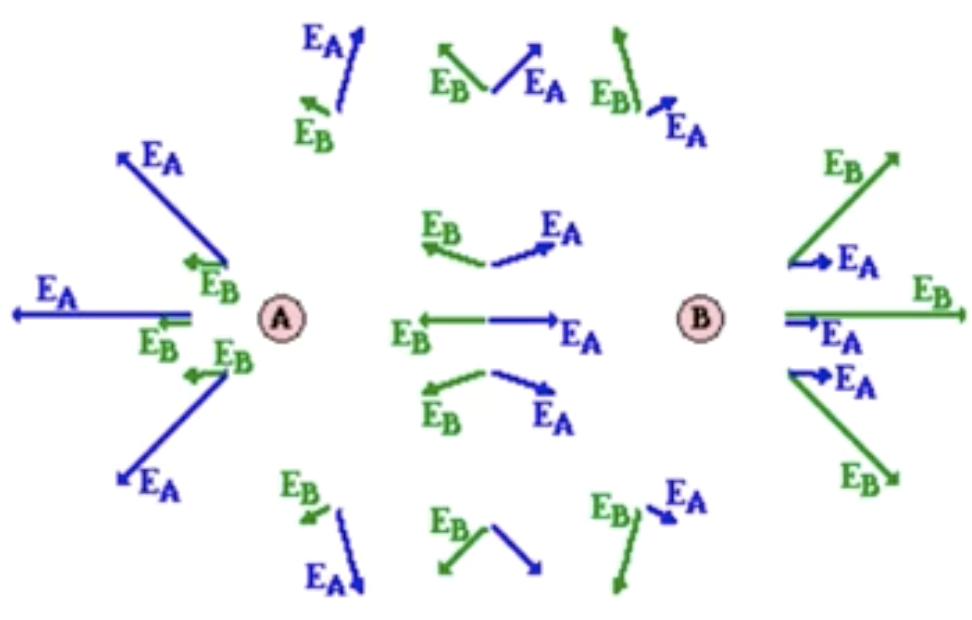
\includegraphics[width=.9\linewidth]{./Screen Shot 2020-08-24 at 9.01.47 PM.png}
\caption{Screen Shot 2020-08-24 at 9.01.47 PM.png}
\end{figure}

In this diagram, A + B are both positive. The diagram, now, shows \emph{both}
electric field vectors for A and B. Take, for instance,

This tidbit: \begin{center}
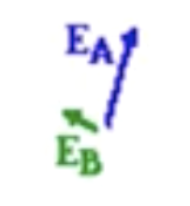
\includegraphics[width=.9\linewidth]{./Screen Shot 2020-08-24 at 9.04.52 PM.png}
\end{center}

If we connected it back to A and B, you will get:

\begin{figure}[htbp]
\centering
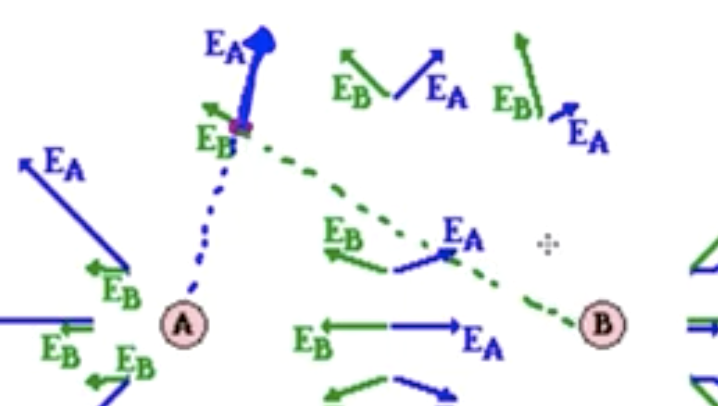
\includegraphics[width=.9\linewidth]{./Screen Shot 2020-08-24 at 9.05.26 PM.png}
\caption{Screen Shot 2020-08-24 at 9.05.26 PM.png}
\end{figure}

As you could see, the force from B is smaller because the point is
farther away from B.

Ok, now, let's see the \emph{net} electric field by adding all of these
vectors up:

\begin{figure}[htbp]
\centering
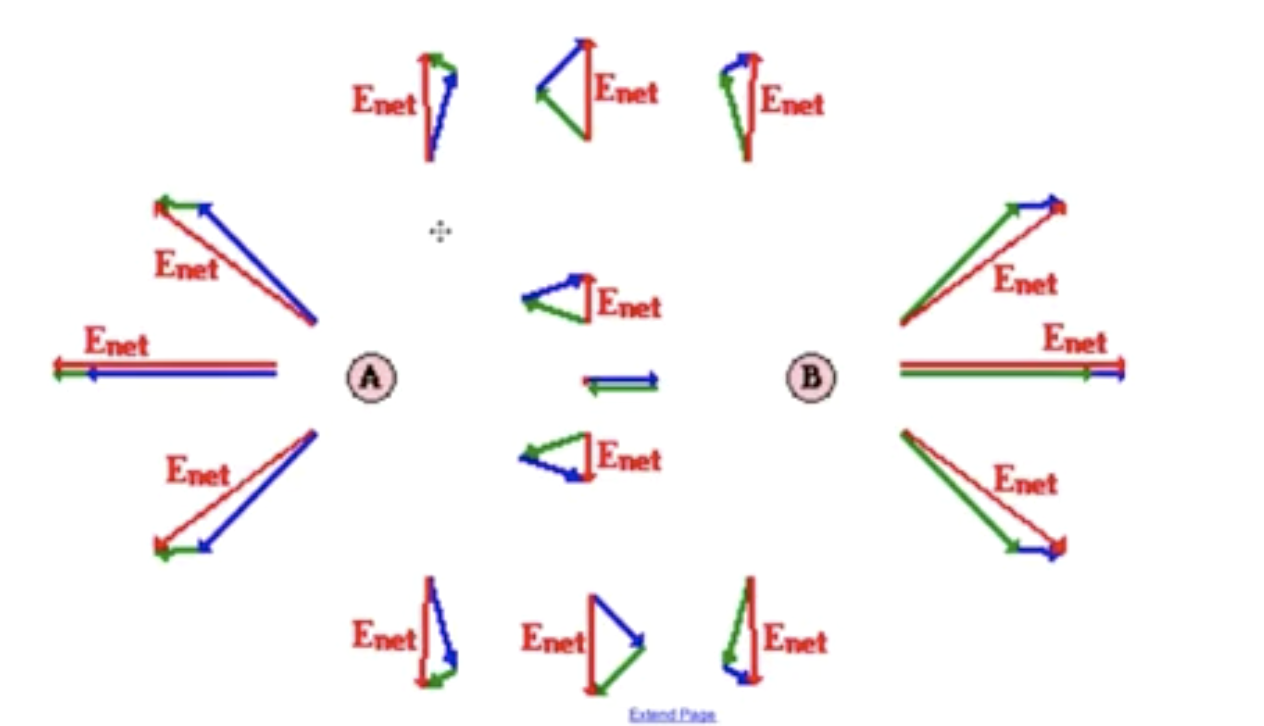
\includegraphics[width=.9\linewidth]{./Screen Shot 2020-08-24 at 9.07.26 PM.png}
\caption{Screen Shot 2020-08-24 at 9.07.26 PM.png}
\end{figure}

Nice! You are, at this point, hopefully seeing something of a symmetry.
Remember how we had two ways of drawing an electric field? That

\begin{enumerate}
\item You choose to draw an infinite amount of vectors, or
\item You draw lines from the center of each element outwards, connecting
all the vectors
\end{enumerate}

If we do option 2, you see this lovely image:

\begin{figure}[htbp]
\centering
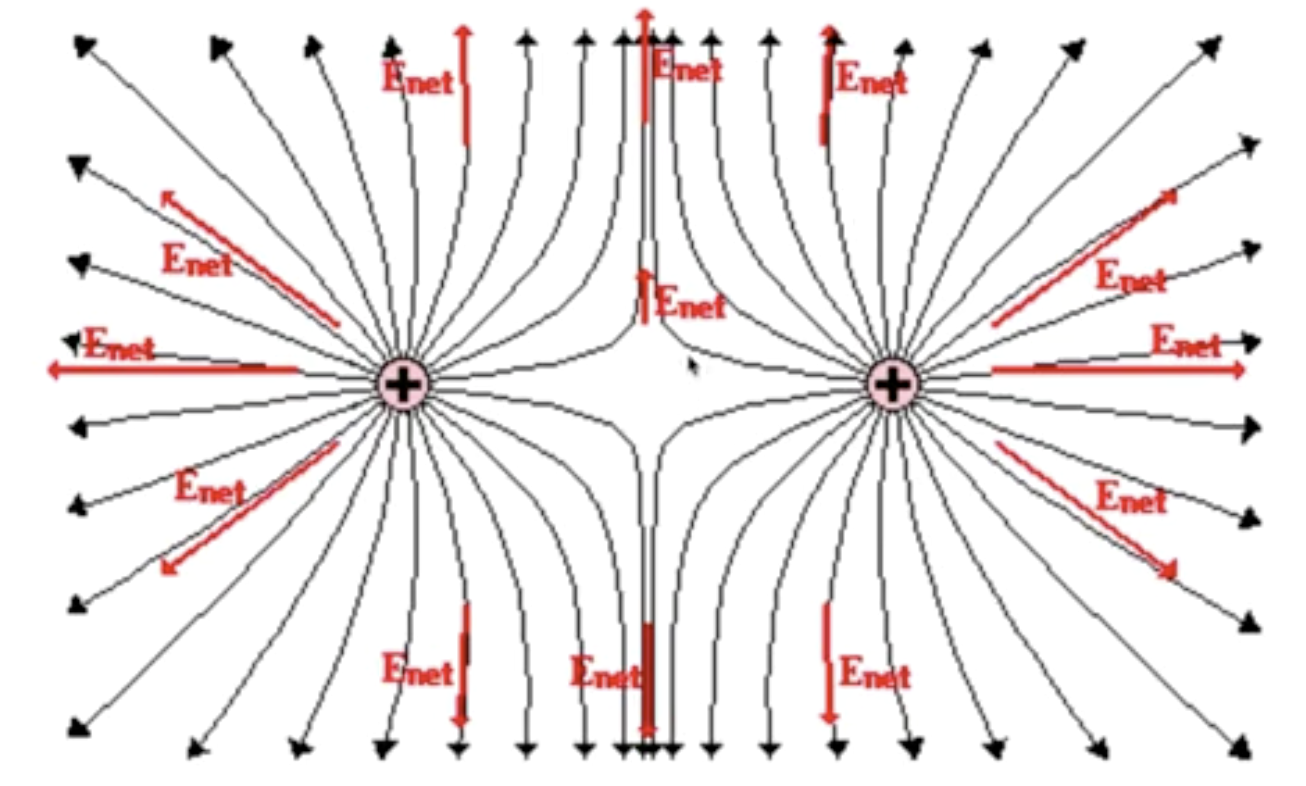
\includegraphics[width=.9\linewidth]{./Screen Shot 2020-08-24 at 9.10.52 PM.png}
\caption{Screen Shot 2020-08-24 at 9.10.52 PM.png}
\end{figure}

Please, be also reminded of the fact that the world is 3D, making the
diagram more like this:

\begin{figure}[htbp]
\centering
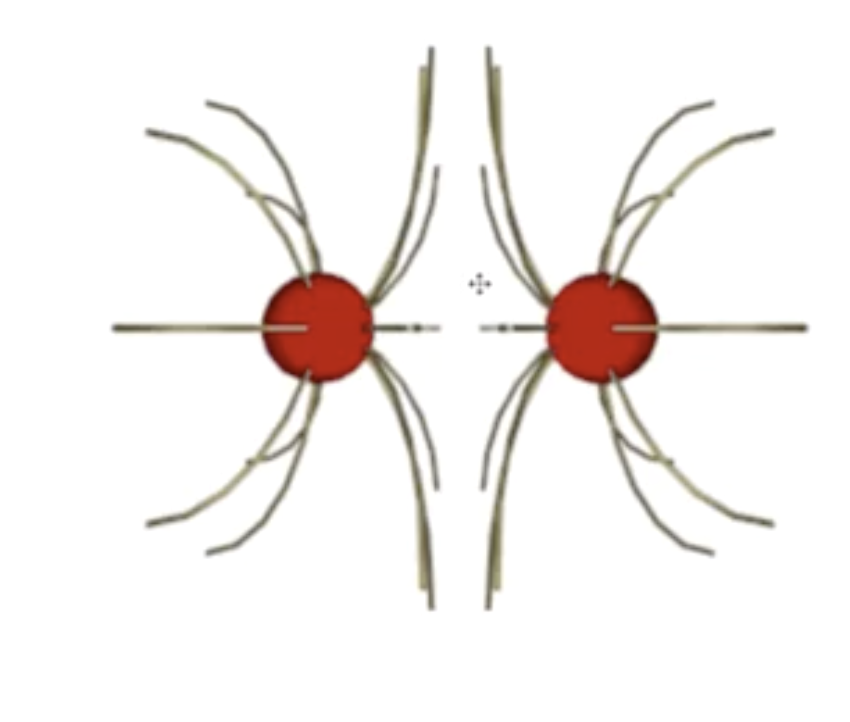
\includegraphics[width=.9\linewidth]{./Screen Shot 2020-08-24 at 9.24.48 PM.png}
\caption{Screen Shot 2020-08-24 at 9.24.48 PM.png}
\end{figure}

Great. Lastly there are other possible configurations of charges apart
from positive-positive, and they are as follows:

\begin{figure}[htbp]
\centering
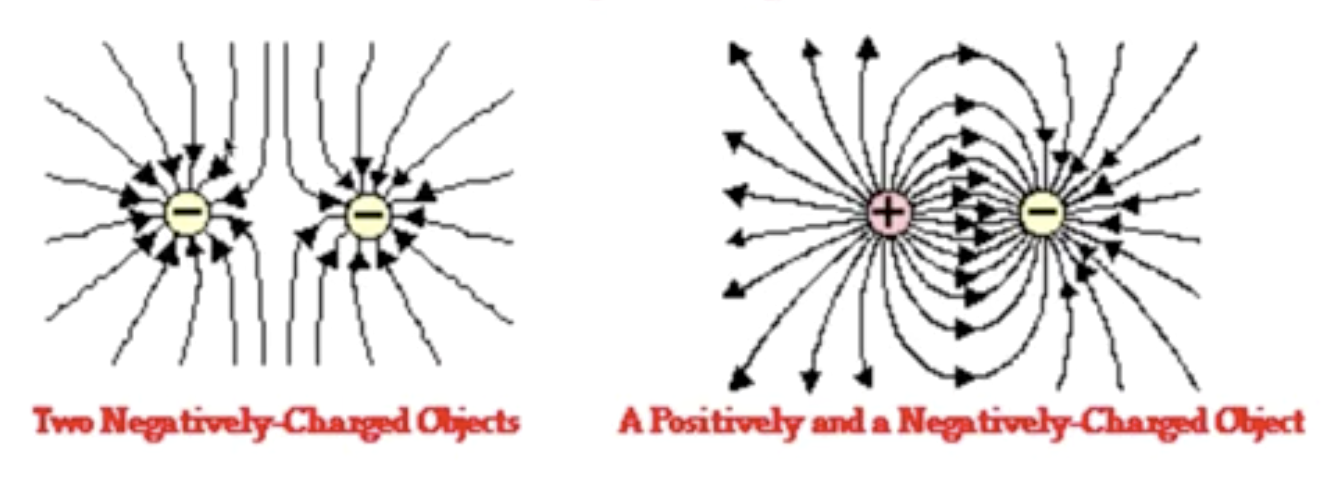
\includegraphics[width=.9\linewidth]{./Screen Shot 2020-08-24 at 9.25.58 PM.png}
\caption{Screen Shot 2020-08-24 at 9.25.58 PM.png}
\end{figure}

As you could see. There is a lovely point (yes, it's actually a point,
but people are lazy and don't to draw, say \emph{infinite} field lines) in
the middle of Neg-Neg and Pos-Pos electric field graphs with a lovely
hole. At that hole, the field value is 0.

(Thanks Mr. Valdez!)

Here's a gallery of electric fields with unequal changes:

\begin{figure}[htbp]
\centering
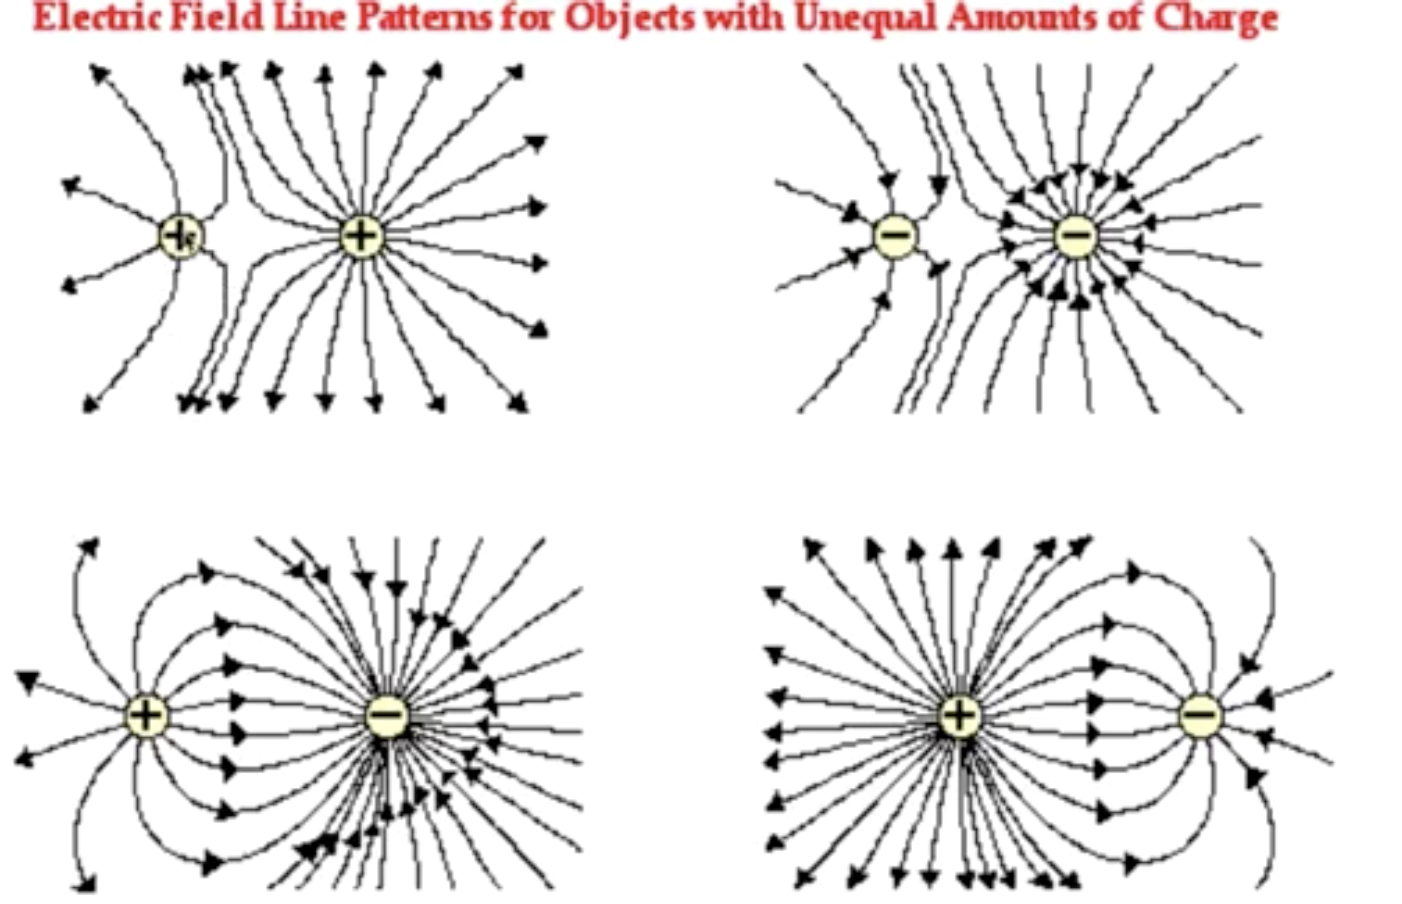
\includegraphics[width=.9\linewidth]{./Screen Shot 2020-08-24 at 9.28.56 PM.png}
\caption{Screen Shot 2020-08-24 at 9.28.56 PM.png}
\end{figure}

As you could see, the higher amount of field lines, the higher is the
strengths. If each charge's field "bends" towards the other,
(i.e. particles that go \emph{AAAAA I AM GOING TO OVERTAKE THE OTHER
PARTICLE'S FIELD LINES})

However, here's something that you should probably remember:

\textbf{Whenever we are analyzing charge fields of multiple changes "together",
remember that we are analyzing the NET electric field.} \emph{Each individual
change does NOT feel its own field.}

This means that, for instance, we drop in a third test charge --- it
WILL change the NET electric field of all three together, but w.r.t. to
the test charge itself, it is only influenced by the net field of the
two others.
\end{document}
